\resizebox{\textwidth}{!}{
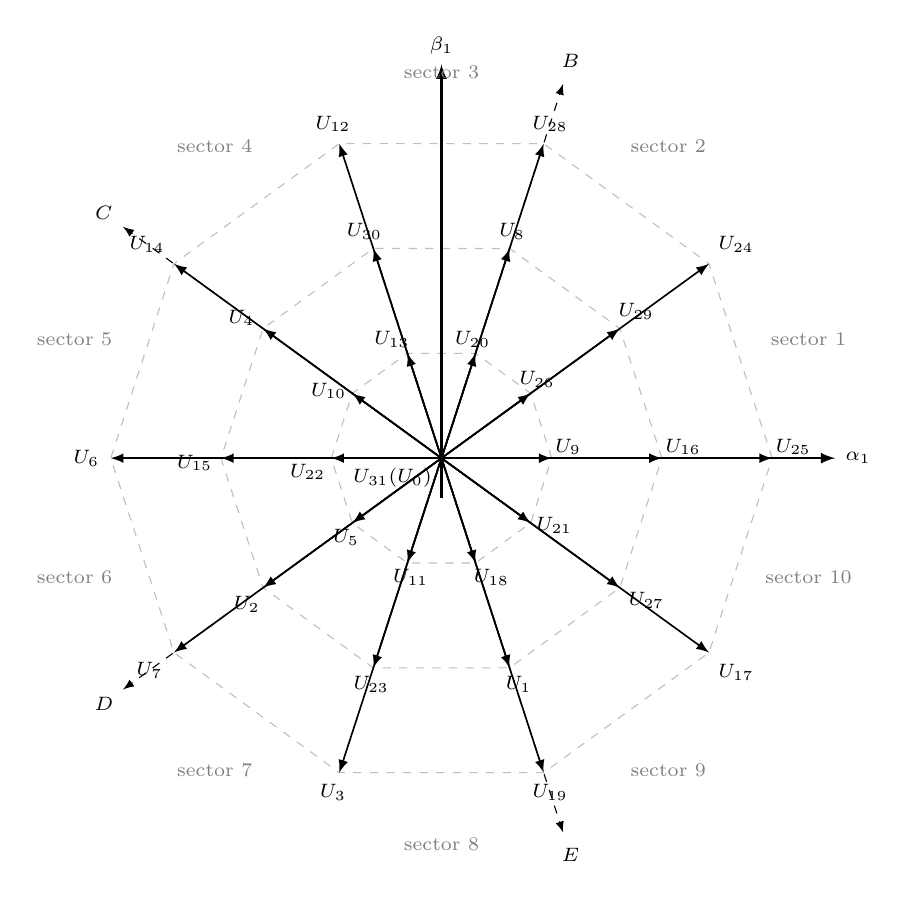
\begin{tikzpicture}[>=latex, font=\scriptsize]

    % Definice poloměrů
    \def\Rone{1.4}   
    \def\Rtwo{2.8}   
    \def\Rthree{4.2} 
    \def\Raxis{5.0}  

    % 1. Kreslení pozadí (čárkované desetiúhelníky)
    \foreach \r in {\Rone, \Rtwo, \Rthree} {
        \draw[dashed, gray!50] (0:\r) \foreach \x in {36,72,...,360} {-- (\x:\r)} -- cycle;
    }

    % 2. Hlavní osy
    \draw[->, thick] (-0.5,0) -- (\Raxis,0) node[right] {$\alpha_1$};
    \draw[->, thick] (0,-0.5) -- (0,\Raxis) node[above] {$\beta_1$};

    % Středový bod
    \node[below left] at (0,0) {$U_{31}(U_0)$};

    % 3. VEKTORY A POPISKY (Sjednocený styl pro osu alfa)

    % VNĚJŠÍ ÚROVEŇ (Level 3)
    \foreach \ang/\lab in {0/U_{25}, 36/U_{24}, 72/U_{28}, 108/U_{12}, 144/U_{14}, 180/U_6, 216/U_7, 252/U_3, 288/U_{19}, 324/U_{17}} {
        \draw[->, semithick] (0,0) -- (\ang:\Rthree);
        % Speciální podmínka pro úhel 0 (osa alfa), aby U25 bylo jako U9
        \ifnum\ang=0
            \node[anchor=south west, inner sep=1pt] at (\ang:\Rthree) {$\lab$};
        \else
            \node[anchor=\ang+180, inner sep=4pt] at (\ang:\Rthree) {$\lab$};
        \fi
    }

    % STŘEDNÍ ÚROVEŇ (Level 2)
    \foreach \ang/\lab in {0/U_{16}, 36/U_{29}, 72/U_8, 108/U_{30}, 144/U_4, 180/U_{15}, 216/U_2, 252/U_{23}, 288/U_1, 324/U_{27}} {
        \draw[->, semithick] (0,0) -- (\ang:\Rtwo);
        \ifnum\ang=0
            \node[anchor=south west, inner sep=1pt] at (\ang:\Rtwo) {$\lab$};
        \else
            \node[anchor=\ang+190, inner sep=3pt] at (\ang:\Rtwo) {$\lab$};
        \fi
    }

    % VNITŘNÍ ÚROVEŇ (Level 1)
    \foreach \ang/\lab in {0/U_9, 36/U_{26}, 72/U_{20}, 108/U_{13}, 144/U_{10}, 180/U_{22}, 216/U_5, 252/U_{11}, 288/U_{18}, 324/U_{21}} {
        \draw[->, semithick] (0,0) -- (\ang:\Rone);
        \ifnum\ang=0
            \node[anchor=south west, inner sep=1pt] at (\ang:\Rone) {$\lab$};
        \else
            \node[anchor=\ang+210, inner sep=2pt] at (\ang:\Rone) {$\lab$};
        \fi
    }

    % 4. Fázové osy a sektory
    \foreach \ang/\name in {72/B, 144/C, 216/D, 288/E} {
        \draw[->, dashed] (0,0) -- (\ang:\Raxis);
        \node at (\ang:\Raxis + 0.3) {$\name$};
    }
    
    \foreach \s/\ang in {1/18, 2/54, 3/90, 4/126, 5/162, 6/198, 7/234, 8/270, 9/306, 10/342} {
        \node[text=gray] at (\ang:\Rthree + 0.7) {sector \s};
    }


\end{tikzpicture}
}